\chapter{Разработка и экспериментальное внедрение системы радиочастотной идентификации}\label{ch:ch5}
Важная задача, возникающая при построении системы радиочастотной идентификации транспортных средств "--- необходимость объединять в реальном времени данные со множества считывателей, которые могут быть размещены на большой территории. Для решения этой задачи была разработана распределенная платформа для интеграции и управления RFID-считывателями. Платформа позволяет интегрировать разрозненные считыватели в единую масштабируемую систему обработки данных.

В 2014--2015 годах был проведён эксперимент в городе Казань, в ходе которого было проведено испытание разработанной платформы и RFID-считывателей для идентификации меток, размещённых на рейсовых автобусах. Весной 2020 года совместно с АО <<Микрон>> в рамках НИР были проведены испытания на полигоне в городе Казань для проверки системы при идентификации меток на автомобилях, движущихся со скоростями до 170~км/ч. Все испытания завершились успешно. Летом 2021 года начались испытания на платном участке центральной кольцевой автодороги (ЦКАД), которые к моменту написания диссертации еще не завершились.

В этой главе приводится описание разработанной платформы и проведенных экспериментальных исследований. В разделе \ref{sec:ch5_architecture} описывается структура платформы управления считывателями и ее основные компоненты, в разделе \ref{sec:ch5_protocols} "--- разработанные протоколы, а в разеделе \ref{sec:ch5_components} "--- модули системы. Далее, в разделе \ref{sec:ch5_implementation}, описывается аппаратная реализация RFID-считывателей и особенности программной реализации. Раздел \ref{sec:ch5_experiments} посвящен описанию экспериментальных исследований разработанных RFID-считывателей и системы управления. Заключение в разделе \ref{sec:ch5_conclusion} завершает главу.

Результаты, представленные в главе, были опубликованы в работах, индексируемых Scoupus/WoS \cite{RFIDCTRL_NETS2CARS2014, RFIDTA2012}. По результатам эксперимента 2020 года был сделан доклад на форуме Kazan Digital Week 2020.
% , и представлены в трудах конференций \cite{RFIDCTRL_DCCN2017, RFIDCTRL_VSPU2014}


%%%%%%%%%%%%%%%%%%%%%%%%%%%%%%%%%%%%%%%%%%%%%%%%%%%%%%%%%%%%%%%%%%%%%%%%%%%%%%%%
\section{Архитектура системы управления считывателями}\label{sec:ch5_architecture}
%%%%%%%%%%%%%%%%%%%%%%%%%%%%%%%%%%%%%%%%%%%%%%%%%%%%%%%%%%%%%%%%%%%%%%%%%%%%%%%%
Радиочастотная идентификация транспорта может применяться для идентификации автомобилей в системах регистрации нарушений правил дорожного движения, для оплаты проезда по платным дорогам, доступа на закрытые территории, а также использоваться при поиске угнанных машин и розыске преступников. Для быстрой реализации различных приложений программное обеспечение должно предоставлять возможность простого добавления новых сервисов в систему, а также обеспечивать масштабируемость.

\begin{figure}[ht]
  \centerfloat{
    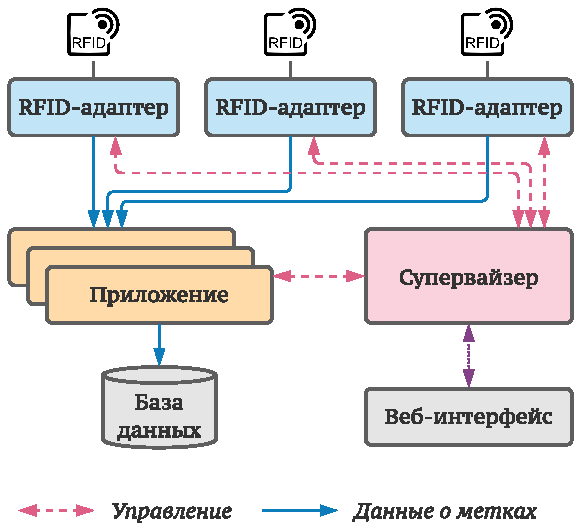
\includegraphics [width=0.5\textwidth]{chapter5/ch5_components}
  }
  \caption{Компоненты системы управления}
  \label{fig:ch5_components}
\end{figure}

Система управления считывателями имеет модульную структуру (см. рис.~\ref{fig:ch5_components}) и включает три типа модулей: супервайзеры, RFID-адаптеры и приложения. Супервайзеры (SVR) отвечают за хранение и управление конфигурацией системы. RFID-адаптеры управляют работой радиомодулей RFID-считывателей, реализуют чтение и запись меток. Приложения обрабатывают потоки прочитанных меток, поступающих от RFID-адаптеров и других приложений. Приложения могут использоваться для объединения потоков от нескольких источников, фильтрации или преобразования протоколов. Кроме перечисленных модулей, в состав системы входят иструменты администрирования "--- консоль и веб-интерфейс.

Каждый модуль системы поддерживает множество объектов, каждый из которых является либо параметром, либо процедурой. Обработка объектов ведётся по запросам, приходящим от пользователей или других модулей системы. Множество объектов полностью определяется типом модуля. Например, каждый RFID--адаптер поддерживает параметры <<температура радио--модуля>>, <<значение Q>>, <<номер сессии>> и процедуры <<выключить радио--модуль>>, <<включить радио--модуль>>. RFID--адаптер, специализированный на поддержке определенного считывателя, может предоставлять объекты, специфичные для конкретной модели считывателя. Каждый модуль получает свои настройки от супервайзера сразу после включения.

Для работы с объектом пользователь или модуль должны отправить запрос супервайзеру через один из поддерживаемых им протоколов управления (рассматриваются ниже). Супервайзер поддерживает множество собственных объектов, например "--- <<число активных пользователей>> или <<статус подключений модулей>>, а также выполняет проксирование объектов всех подключенных модулей. Когда супервайзер получает запрос на объект, который не принадлежит ему самому, он перенаправляет запрос модулю, которому этот объект принадлежит, и отвечает клиенту, перенаправляя ответ, полученный от модуля.

В системе используется разделение потоков данных и управления: все управление производится через супервайзер, а данные передаются напрямую между RFID-адаптерами и приложениями. Такое разделение позволяет, с одной стороны, снизить нагрузку на супервайзер и увеличить масштабируемость, а с другой "--- использовать более простые протоколы между компонентами. Так как основное назначение системы "--- непрерывное чтение меток проезжающих автомобилей, передача данных о прочитанных метках организована в виде потоков. Приложение, которое хочет получать данные о метках от RFID-адаптера или другого приложения должно подписаться на поток.

Пользователи могут настраивать систему и взаимодействовать с RFID-адаптерами и приложениями. В системе определены четыре уровня доступа: наблюдатели, операторы, администраторы и суперпользователи. Наблюдатели могут подписываться на потоки меток, но не могут записывать метки или менять настройки оборудования. Операторы имеют право настраивать RFID--адаптеры и выполнять операции чтения/записи меток, но не могут менять настройки остальных компонентов системы. Администраторы имеют право настраивать модули, но не могут записывать метки. Суперпользователи имеют права на любые действия с системой. Помимо уровней доступа пользователей с каждым компонентом связан специальный системный уровень доступа, который позволяет ему работать с определенным набором объектов других компонентов. Например, приложения могут читать, но не имеют права записывать параметры RFID--адаптеров.

Поскольку все модули системы взаимодействуют друг с другом по сети, физически они могут располагаться где угодно. Типичные примеры размещений модулей показаны на рис.~\ref{fig:ch5_deployments}.

\begin{figure}[ht]
  \centerfloat{
    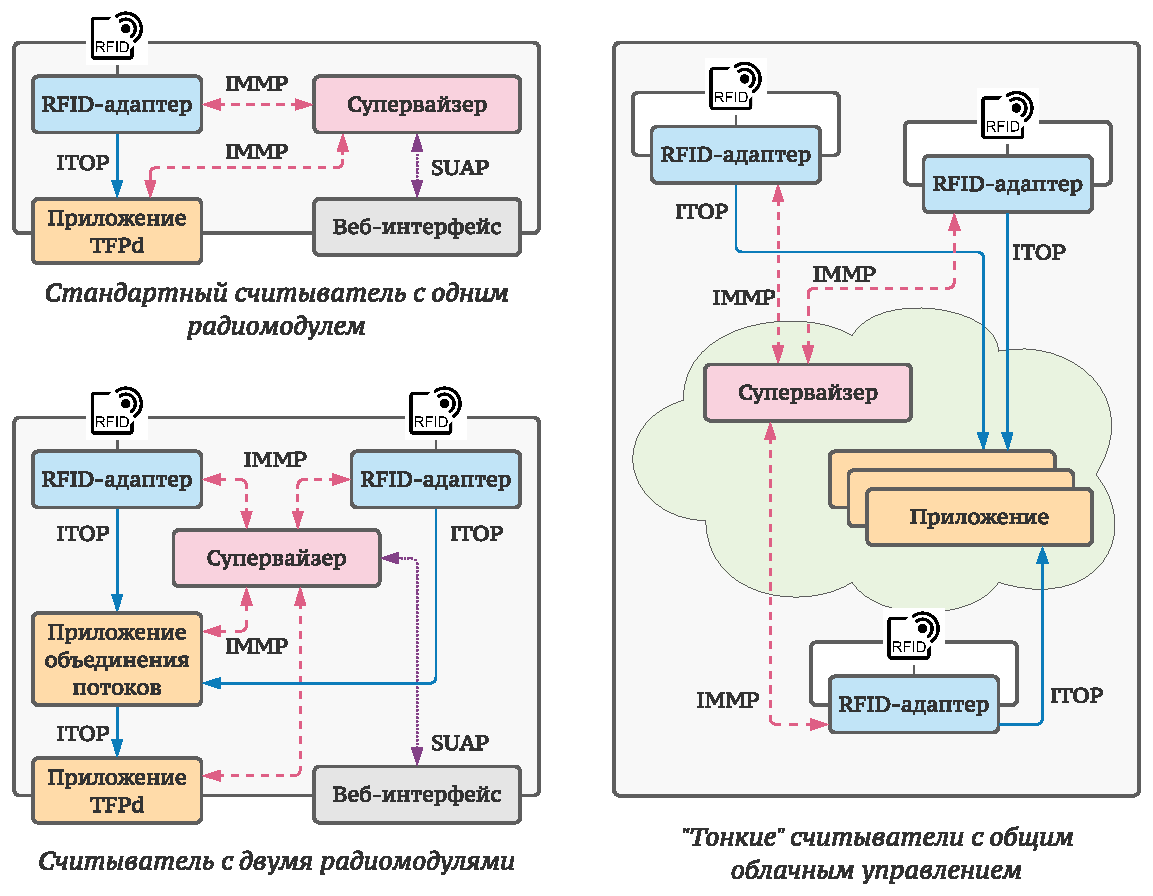
\includegraphics [width=0.9\textwidth]{chapter5/ch5_deployments}
  }
  \caption{Примеры размещения модулей системы}
  \label{fig:ch5_deployments}
\end{figure}

Для обычного RFID--считывателя, построенного на базе среднего процессора (например, одноядерный ARM A7 или ARM A8), обладающего небольшим объемом оперативной памяти порядка 256--512~МБ и имеющего в составе один радиомодуль, достаточно установить супервайзер, RFID-адаптер, а также приложение для подключения к потоку прочитанных меток снаружи (TFPD) и модуль, предоставляющий доступ к настройке считывателя через веб-интерфейс или консоль. Такое размещение компонентов позволяет передавать данные обо всех прочитанных метках в центр обработки данных и, при необходимости, реализовывать операции чтения/записи через подключение внешних модулей и пользователей. Именно такая конфигурация считывателей использовалась во всех проведенных экспериментах.

Если считыватель имеет более мощное вычислительное ядро, на нём можно разместить несколько приложений. Например, на нем можно установить приложения для фильтрации прочитанных меток или нахождения соответствий с номерными знаками, распознанными камерами. Если считыватель включает несколько радиомодулей, то потребуется несольких RFID--адаптеров. Хотя каждый компонент системы не требователен к вычислительным ресурсам по отдельности, для выполнения задач обработки потоков меток могут потребоваться дополнительные ресурсы. Желательно использовать 2-х или 4-х ядерный процессор ARM и 512 "--- 1024 МБ оперативной памяти.

В наиболее сложном случае система может работать в распределенном режиме, а различные ее компоненты размещаться на считывателях и серверах, при этом считыватели могут быть сделаны чрезвычайно <<тонкими>> "--- на них достаточно разместить RFID--адаптер, который будет подключаться по сети к супервайзеру, работающему на внешнем сервере или в облаке. Приложения также могут работать на отдельных физических или виртуальных внешних серверах. В этом варианте считыватели могут быть реализованы на самых простых вычислительных компонентах, что позволит снизить их стоимость, а приложения и супервайзер выполняются в центре обработки данных на мощном вычислительном оборудовании, благодаря чему им можно поручить работу с большим числом считывателей. Такой вариант размещения наиболее гибок и позволяет построить распределенную систему, состоящую из сотен считывателей, каждый из которых может администрироваться из единой консоли.



%%%%%%%%%%%%%%%%%%%%%%%%%%%%%%%%%%%%%%%%%%%%%%%%%%%%%%%%%%%%%%%%%%%%%%%%%%%%%%%%
\section{Протоколы взаимодействия компонентов системы}\label{sec:ch5_protocols}
%%%%%%%%%%%%%%%%%%%%%%%%%%%%%%%%%%%%%%%%%%%%%%%%%%%%%%%%%%%%%%%%%%%%%%%%%%%%%%%%

В системе управления передача данных и управления разделены. Для упрвления системой были разработаны протоколы IMMP (Internal Modules Management Protocol) и SUAP (Simple User Access Protocol), а для передачи потоков меток и работы с радиомодулями "--- протоколы ITOP (Internal Tags Operation Protocol) и TFP (Tag Flow Protocol). Протоколы IMMP и ITOP используются для управления и передачи внутри системы, а протоколы SUAP и TFP "--- для работы работы с супервайзером со стороны интерфейсов управления и получения потоков прочитанных меток во внешние информационные системы. Все протоколы, используемые в системе, показаны на рис.~\ref{fig:ch5_protocols}.

\begin{figure}[ht]
  \centerfloat{
    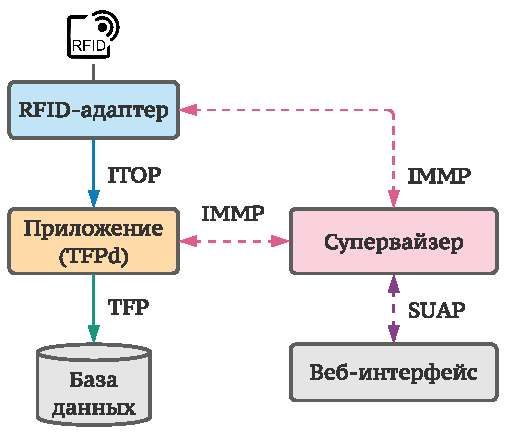
\includegraphics [width=0.4\textwidth]{chapter5/ch5_protocols}
  }
  \caption{Протоколы передачи данных и управления}
  \label{fig:ch5_protocols}
\end{figure}

Все протоколы имеют клиент--серверную архитектуру, соединение создаётся клиентом. Каждый запрос должен подтверждаться получателем с помощью специального сообщения Response, содержащего результат обработки запроса или код ошибки. Запросы упорядочиваются с помощью порядкового номера ReqSN (Request Sequence Number): клиент и сервер поддерживают счетчики, перед отправкой значение счетчика увеличивается и помещается в соответствующее поле в запросе. В ответе на запрос поле ReqSN должно совпадать со значением счетчика из запроса. Этот механизм позволяет реализовать асинхронную обработку запросов "--- отправителю запроса не нужно ждать ответа для того, чтобы передать новый запрос. При этом отправитель может быть уверен, что запросы будут обработаны в порядке их передачи: если получатель видит, что номер запроса меньше последнего обработанного, запрос будет проигнорирован. С каждым запросом также связано максимальное ожидание ответа, после которого отправитель считает, что запрос не был выполнен.

Формат сообщений, кодируемых с помощью ASCII-строк, аналогичен форматам, используемым в HTTP v1.1 и SIP.


%%% --------------------------------------------
\subsection{IMMP "--- протокол управления модулями}\label{sec:ch5_immp}
%%% --------------------------------------------

Протокол IMMP работает поверх транспортного уровня TCP и реализует функции получения модулями своей начальной конфигурации от супервайзера, получения и установки значений параметров модулей, а также удалённый вызов процедур. В роли сервера всегда выступает супервайзер, а клиента "--- один из модулей системы.

В протоколе определены семь запросов: HELLO, ACK, BYE, GET, SET и CALL. Запрос HELLO отправляется клиентом для создания соединения. Если соединение может быть установлено, сервер (супервайзер) сначала передает ответ с кодом успеха (200), а затем "--- запрос ACK, в котором передает конфигурацию модуля и случайный ключ сессии (SKey, Session Key), по которому в дальнейшем он будет авторизовывать запросы этого клиента. Запросы GET и SET используются для чтения и записи значений объектов--параметров, а запрос CALL "--- для удаленного вызова процедур. Запросы GET, SET и CALL могут передаваться как клиентом, так и сервером.

\begin{figure}[ht]
  \centering
  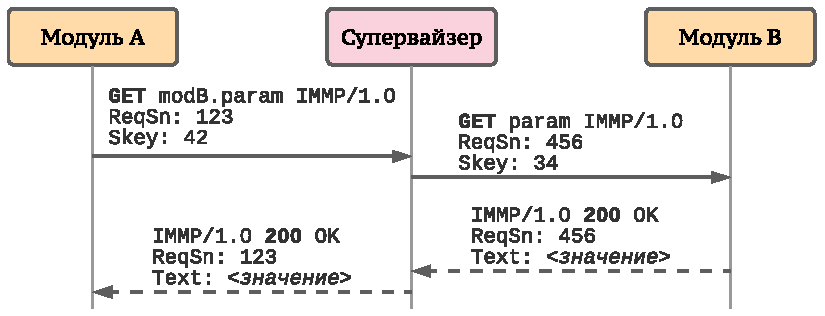
\includegraphics [width=0.7\textwidth] {chapter5/ch5_immp_proxy}
  \caption{Работа супервайзера в режиме IMMP-прокси}
  \label{fig:ch5_immp_proxy}
\end{figure}

Если супервайзеру нужно выполнить какую-либо операцию над объектом другого модуля, он передает соответствующий запрос (GET, SET или CALL). Если же модулю A нужно выполнить действие над объектом модуля B, то супервайзер выступает в роли прокси-сервера: модуль A передает запрос супервайзеру, который тот передает модулю B, дожидается ответа и пересылает его обратно модулю A (см. рис.~\ref{fig:ch5_immp_proxy}).

\begin{figure}[ht]
  \centering
  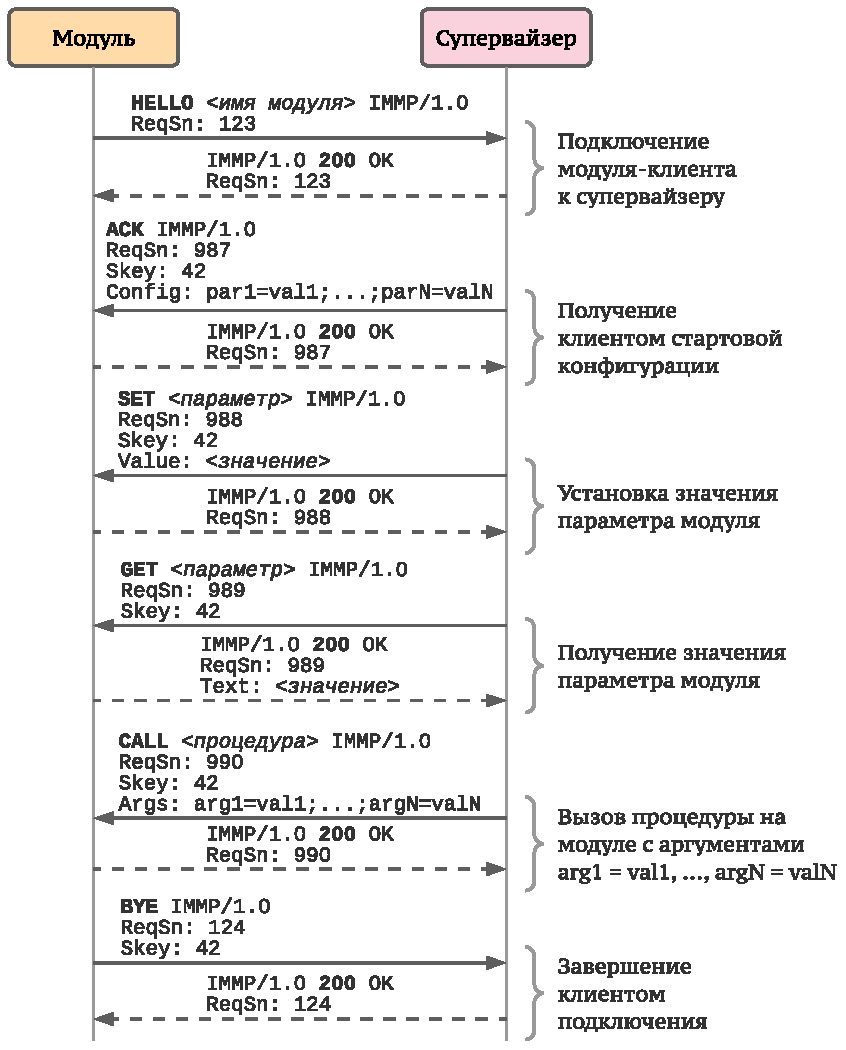
\includegraphics [width=0.70\textwidth] {chapter5/ch5_immp_session}
  \caption{Пример IMMP-сессии}
  \label{fig:ch5_immp_session}
\end{figure}

Пример соединения показан на рис.~\ref{fig:ch5_immp_session}. Клиент передает запрос HELLO со своим именем, сервер отвечает кодом 200. Затем супервайзер готовит стартовую конфигурацию клиента и передает ее в запросе ACK, получение которого клиент должен подтвердить. Такое разделение ответов сервера возникает из-за того, что при высокой нагрузке на супервайзер подготовка стартовой конфигурации может занять время, которое может превышать время ожидания ответа на запрос HELLO. После получения ответа на HELLO клиент может ждать гораздо дольше получения своей конфигурации в ACK. Помимо начальной конфигурации, в ACK супервайзер передает ключ сессии SKey, который используется в дальнейшем обмене сообщениями. После обмена запросами HELLO и ACK начинается основная часть сессии. В ней клиент и сервер обмениваются запросами GET, SET и CALL. Завершает сессию в этом примере клиент отправкой запроса BYE.



%%% --------------------------------------------
\subsection{SUAP "--- протокол подключения интерфейсов управления}\label{sec:ch5_suap}
%%% --------------------------------------------

Протокол SUAP представляет собой упрощенную версию IMMP, работающую через UDP. Он предназначен для подключения пользовательских интерфейсов к супервайзеру. В функции SUAP входят получение и установка значений параметров и удаленный вызов процедур. Протокол не содержит запроса ACK и не является симметричным "--- запросы GET, SET и CALL могут передаваться только от клиента серверу. Кроме этого, есть некоторые отличия в кодировании ответов: если в IMMP значение параметра в ответе на запрос GET передается в поле заголовка Text, то в SUAP значение параметра содержится в теле ответа, отделенном пустой строкой от последнего заголовка.

\begin{figure}[ht]
  \centering
  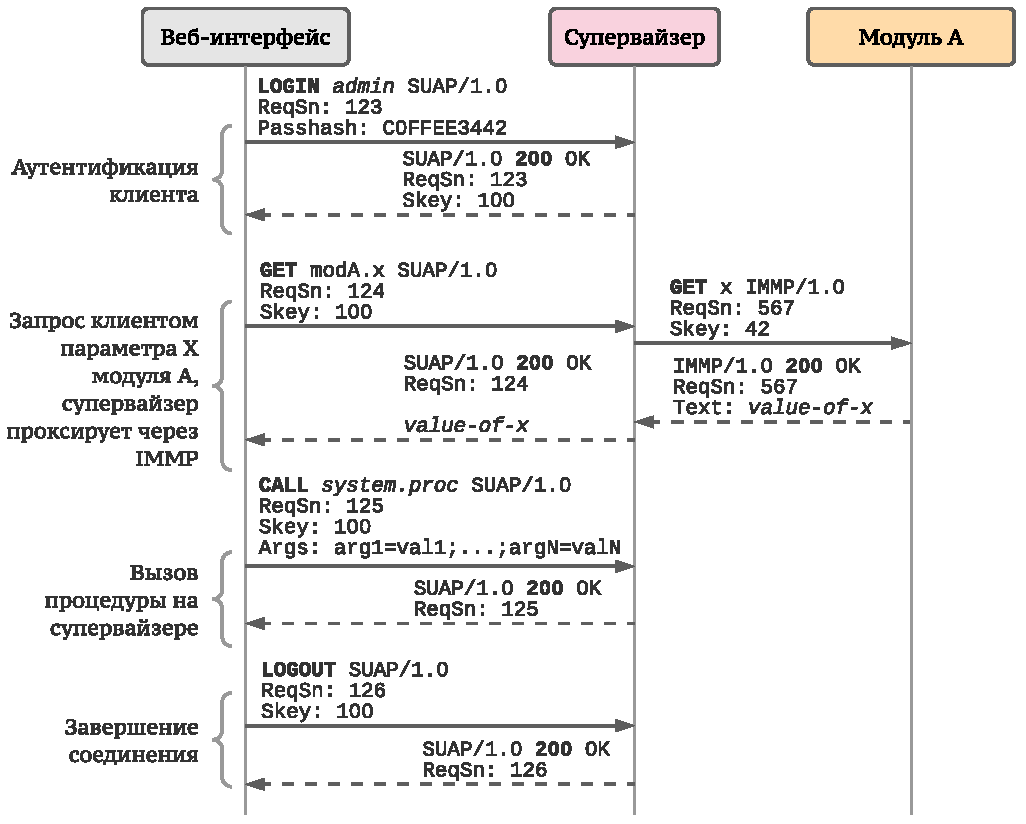
\includegraphics [width=0.85\textwidth] {chapter5/ch5_suap_session}
  \caption{Пример SUAP-сессии}
  \label{fig:ch5_suap_session}
\end{figure}

Аутентификация пользователей производится с помощью логина и пароля. Пароль может передаваться либо нешифрованным текстом, либо в виде хеша. В отличие от IMMP, вместо запроса HELLO клиент в начале сессии должен отправить запрос LOGIN, а для заврешения сессии "--- запрос LOGOUT. Ключ сессии (SKey) используется для авторизации запросов клиента и передается супервайзером в ответе на запрос LOGIN. Пример сессии SUAP показан на рис.~\ref{fig:ch5_suap_session}.

Отметим, что использование SKey для авторизации запросов не является безопасным: если злоумышленник сможет перехватить UDP-пакеты SUAP-сессии, то он сможет получить значение SKey и выполнять операции над системой с уровнем доступа скомпрометированного пользователя. Вопросы обеспечения защиты информации в системе управления требуют дальнейшей разработки, возможные решения "--- использование DTLS (Datagram Transport Layer Security), замена SUAP на HTTPS и реализация REST API на супервайзере или замена SUAP на gRPC с защитой SSL/TLS.



%%% --------------------------------------------
\subsection{ITOP "--- протокол работы с RFID-адаптерами}\label{sec:ch5_itop}
%%% --------------------------------------------

Протокол предназначен для связи между модулями системы (приложениями и RFID-адаптерами), желающими осуществлять действия над метками. Он позволяет читать и записывать память меток, а также подписываться на потоки считанных меток. Подписка может быть позднее отменена, также она завершается при закрытии соединения любой из сторон.

В протоколе определены семь запросов: HELLO, BYE, READMEM, WRITEMEM, WRITEEPC, SUBSCRIBE, UNSUBSCRIBE. Сервер может передать запрос BYE, остальные запросы передаются только клиентом. Запросы HELLO и BYE используются для создания и завершения соединений. SUBSCRIBE и UNSUBSCRIBE используются для создания и отмены подписки, а запросы READMEM, WRITEMEM и WRITEEPC "--- для чтения или записи данных на заданную метку.

Когда клиент хочет установить ITOP-соединение, он передает серверу запрос HELLO. В этот запрос клиент включает значение SKey, полученное ранее при создании IMMP- или SUAP--соединения. Значение SKey используется для авторизации сервером действий клиента. Например, администраторы и наблюдатели не имеют права записывать метки, а единственная разрешенная им операция "--- создание подписки на получение потока меток. Для авторизации сервер перед выполнением любой из операций READMEM, WRITEMEM, WRITEEPC или SUBSCRIBE вызывает процедуру супервайзера <<system.auth-tagop>> с помощью CALL-запроса IMMP и передает в качестве ее аргументов ключ SKey клиента и тип операции. Если супервайзер подтвердит право клиента на запрошенное действие, то сервер выполнит операцию, в противном случае сообщит клиенту о ее недоступности. Для завершения соединения клиент или сервер отправляют запрос BYE. Пример сессии между веб-интерфейсом, пользователь которого ранее авторизовался с помощью SUAP и получил ключ SKey, и RFID-адаптером показан на рис.~\ref{fig:ch5_itop_session_1}.

\begin{figure}[ht]
  \centerfloat{
    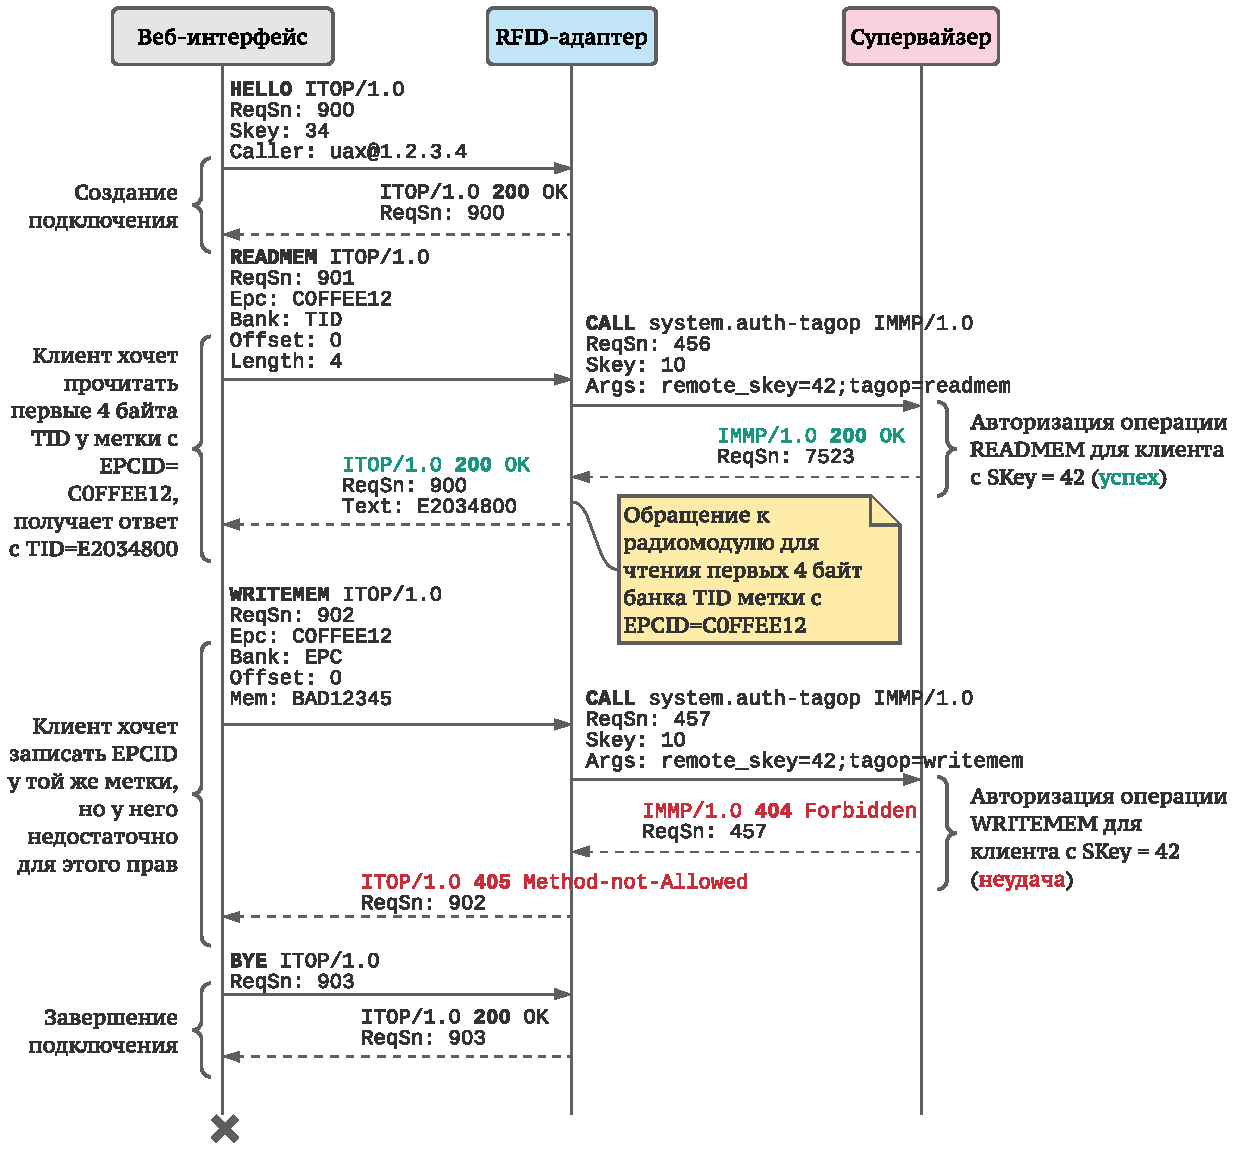
\includegraphics [width=0.9\textwidth] {chapter5/ch5_itop_session_1}
  }
  \caption{Пример соединения ITOP между веб-интерфейсом и RFID-адаптером}
  \label{fig:ch5_itop_session_1}
\end{figure}

Кроме чтения и записи меток по запросу протокол ITOP позволяет создавать подписки на считанные метки. Если клиент желает непрерывно получать информацию о прочитанных метках от сервера, он передает запрос SUBSCRIBE. Как только считывается (если сервер "--- RFID-адаптер) или принимается (если сервер "--- приложение) новая метка, сервер асинхронно передает специальное сообщение NOTIFY клиенту, содержащее информацию о метке. Когда клиент желает остановить получение потока, он отменяет подписку передачей запроса UNSUBSCRIBE. Если клиент (например, веб-интерфейс) хочет читать метки только в течение заданного интервала, то он может добавить в запрос SUBSCRIBE заголовок Continuous со значением false и указать длительность чтения в миллисекундах в заголовке Duration. В этом случае клиенту не нужно явно завершать подписку отправкой UNSUBSCRIBE, она завершится автоматически по истечении заданного времени. Пример создания подписок двумя приложениями показан на рис.~\ref{fig:ch5_itop_session_2}. В этом примере приложение A создает подписку с автоматическим продлением и завершает ее явно, а приложение B читает метки только в течение 0,5~секунд.

\begin{figure}[ht]
  \centerfloat{
    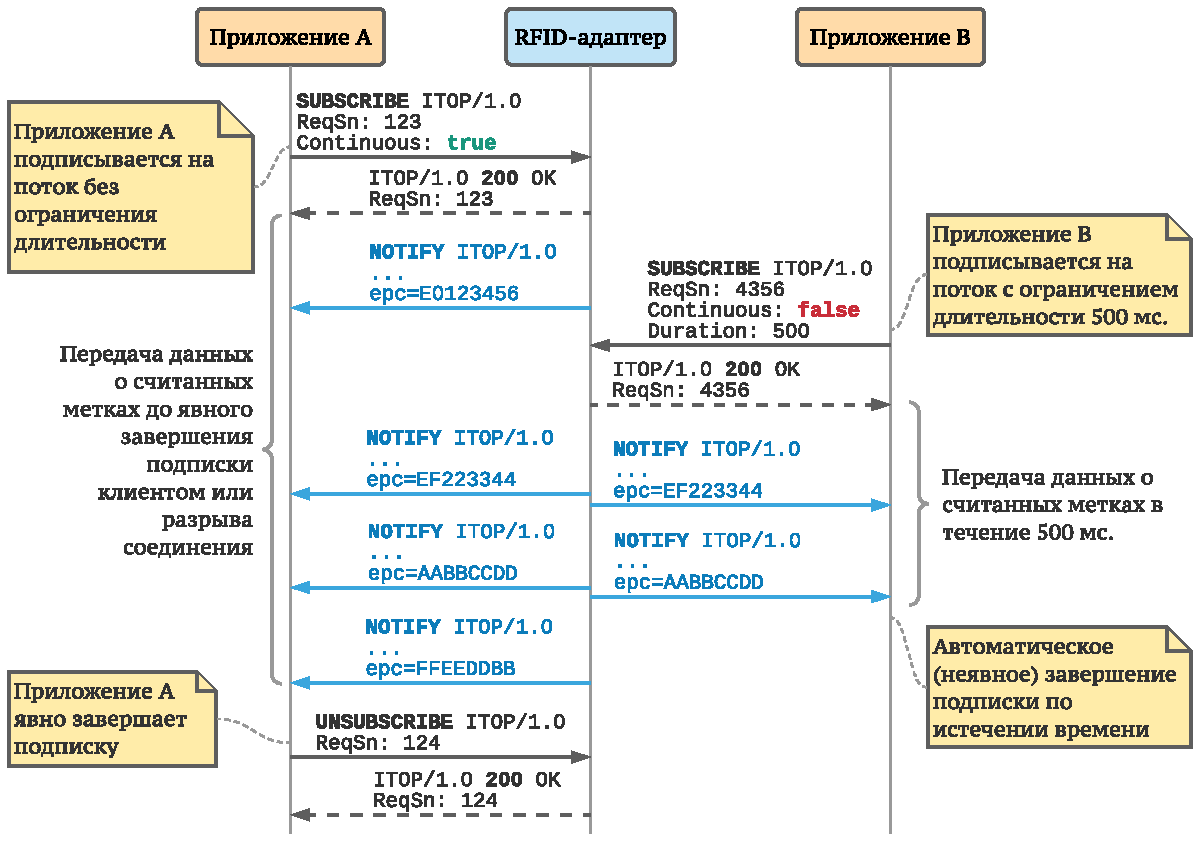
\includegraphics [width=0.9\textwidth] {chapter5/ch5_itop_session_2}
  }
  \caption{Пример создания подписок в соединении ITOP}
  \label{fig:ch5_itop_session_2}
\end{figure}

Тело сообщения NOTIFY может содержать следующие поля:

\begin{itemize}
	\item epc: значение EPC прочитанной метки;
	\item tid: значение банка TID прочитанной метки;
	\item power: мощность принятого сигнала;
	\item antenna: номер антенны, на которой была считана метка;
	\item frequency: частота, на которой работал считыватель;
	\item count: число раз, которое метка была считана;
	\item um: содержимое банка памяти USER MEMORY;
	\item source: имя RFID--адаптера, считавшего метку;
	\item id: идентификатор метки.
\end{itemize}

Поле id может заполняться данными, специфичными для приложения, например "--- значением EPC или номером транспортного средства, полученным приложением с помощью обращения к базе данных по TID или в резлультате декодирования EPCID. Поле um используется только при чтении банка пользовательской памяти, а поле source нужно только при использовании нескольких RFID-адаптеров. Если какие-то из полей не содержат данных, их можно опустить. Значение каждого поля передается в отдельной строке, общее число строк содержится в заголовке Content-length.

Если в роли сервера выступает не RFID-адаптер, а приложение, то оно может не поддерживать некоторые из операций, например WRITEMEM, WRITEEPC или READMEM. В этом случае в ответ на недоступные запросы оно будет передавать клиенту код 405 (Method-not-Allowed).

Так как радиомодуль не может одновременно выполнять несколько операций, ключевая сложность в реализации ITOP-сервера для RFID-адаптера заключается в правильном мультиплексировании. Для этого потребовалось разработать алгоритм обработки запросов клиентов, позволяющий исключить блокировки и обеспечить такой уровень задержек, чтобы даже при наличии активных подписок другие пользователи могли выполнять свои операции чтения, записи или изменения настроек радиомодуля. Подробнее реализацию RFID-адаптера рассмотрим в разделе~\ref{sec:ch5_components_g2rd}.


%%% --------------------------------------------
\subsection{TFP "--- протокол потокового чтения меток}\label{sec:ch5_tfp}
%%% --------------------------------------------

Протокол TFP является упрощенной версией протокола ITOP и предназначен для получения данных о метках из пользовательских интерфейсов или внешних клиентов. Например, TFP-клиенты могут записывать данные о прочитанных метках в базу данных или отправлять во внешнюю информационную систему по REST API или gRPC. Специальное приложение TFP Daemon (TFPD) выступает в роли моста между ITOP и TFP: с одной стороны это приложение выступает в роли сервера протокола TFP, с другой "--- клиента ITOP. В протоколе TFP поддерживается только механизм создания подписок, прочие функции (запись меток, чтение заданных областей памяти и пр.) он не реализует. Протокол поддерживает запросы HELLO, BYE, SUBSCRIBE и UNSUBSCRIBE, данные о метках передаются, как и в ITOP, в сообщениях NOTIFY. Пример сессии TFP приведен на рис.~\ref{fig:ch5_tfp_session_1}.

\begin{figure}[ht]
  \centerfloat{
    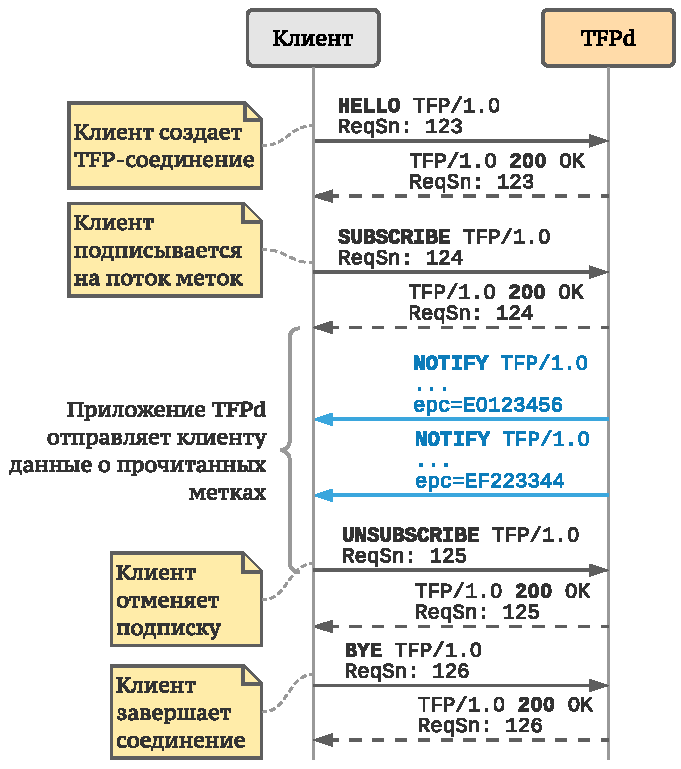
\includegraphics [width=0.5\textwidth] {chapter5/ch5_tfp_session_1}
  }
  \caption{Пример подключения клиента по протоколу TFP}
  \label{fig:ch5_tfp_session_1}
\end{figure}

Использование TFP-сервера позволяет снизить нагрузку на RFID-адаптер и на супервизор при одновременном подключении множества клиентов. Сервер TFP создает ITOP-подписку только в том случае, если к нему подключен хотя бы один клиент и этот клиент подписан. Если подписанных клиентов несколько, TFP-серверу достаточно одной ITOP-подписки, данные из которой он будет пересылать всем клиентам. Когда последний клиент отменяет подписку или отключается, TFP-сервер завершает ITOP-подписку и, если других запросов по ITOP-соединениям у RFID-адаптера нет, он может выключить радиомодуль до появления новых клиентов. Пример работы TFP-сервера с несколькими клиентами приведен на рис.~\ref{fig:ch5_tfp_session_2}.

\begin{figure}[ht]
  \centerfloat{
    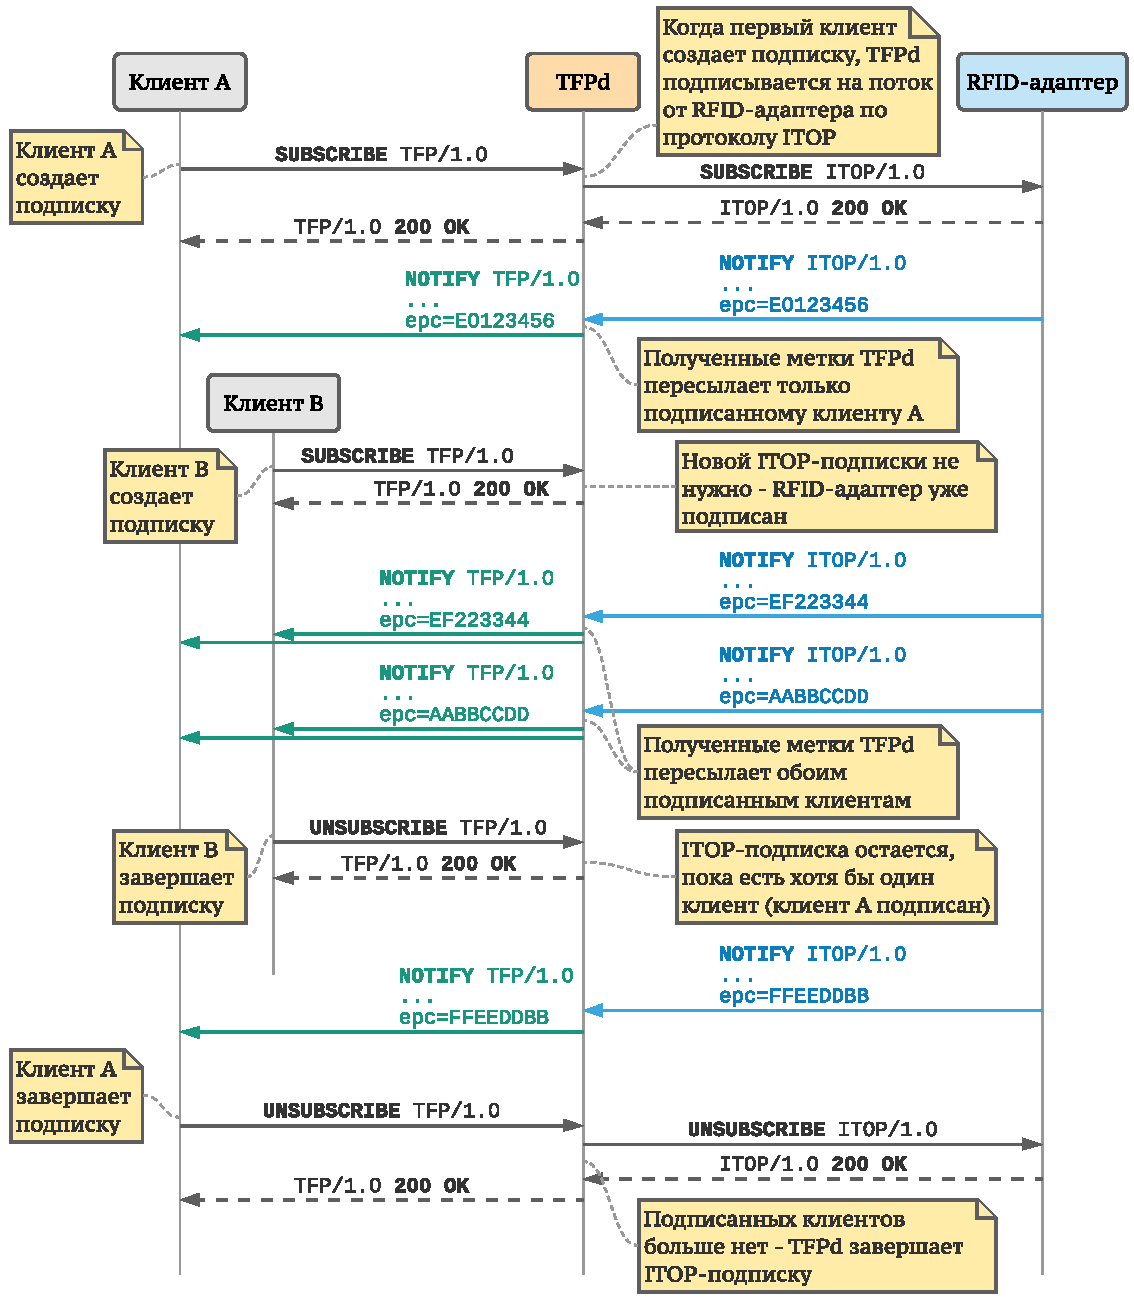
\includegraphics [width=0.9\textwidth] {chapter5/ch5_tfp_session_2}
  }
  \caption{Работа TFP-сервера при создании подписок от двух клиентов}
  \label{fig:ch5_tfp_session_2}
\end{figure}



%%%%%%%%%%%%%%%%%%%%%%%%%%%%%%%%%%%%%%%%%%%%%%%%%%%%%%%%%%%%%%%%%%%%%%%%%%%%%%%%
\section{Основные компоненты системы}\label{sec:ch5_components}
%%%%%%%%%%%%%%%%%%%%%%%%%%%%%%%%%%%%%%%%%%%%%%%%%%%%%%%%%%%%%%%%%%%%%%%%%%%%%%%%

Ключевыми компонентами системы являются супервизор (SVR), модуль управления радиомодулем RFID (G2RD), приложение TFPD и утилита UAX, выполняющая функции SUAP- и ITOP-клиента. Также в состав системы управления входят служебные компоненты "--- клиент TFPC, веб-интерфейс и консольные интерфейсы, которые используют UAX для отправки запросов SVR по SUAP и RFID-адаптеру по ITOP, а также специальная программа RRRD (Road RFID Reader Daemon), управляющая запуском остальных компонентов. Рассмотрим эти компоненты подробнее.


%%% --------------------------------------------
\subsection{Супервизор SVR}\label{sec:ch5_components_svr}
%%% --------------------------------------------

Супервизор управляет работой всех остальных модулей. Его основные задачи: аутентификация пользователей и модулей, передача запросов получения и установки параметров и вызова процедур на модулях системы, хранение и передача начальной конфигурации подключенным модулям, а также реализация логического интерфейса для взаимодействия с операционной системой (например, настройка сетевого интерфейса). SVR выполняет роль IMMP-сервера, при получении запросов относительно параметров других модулей он выполняет функции прокси-сервера (см. рис.~\ref{fig:ch5_immp_proxy}). Также SVR выполняет роль SUAP-сервера для обслуживания запросов со стороны пользовательских интерфейсов.

\begin{figure}[ht]
  \centerfloat{
    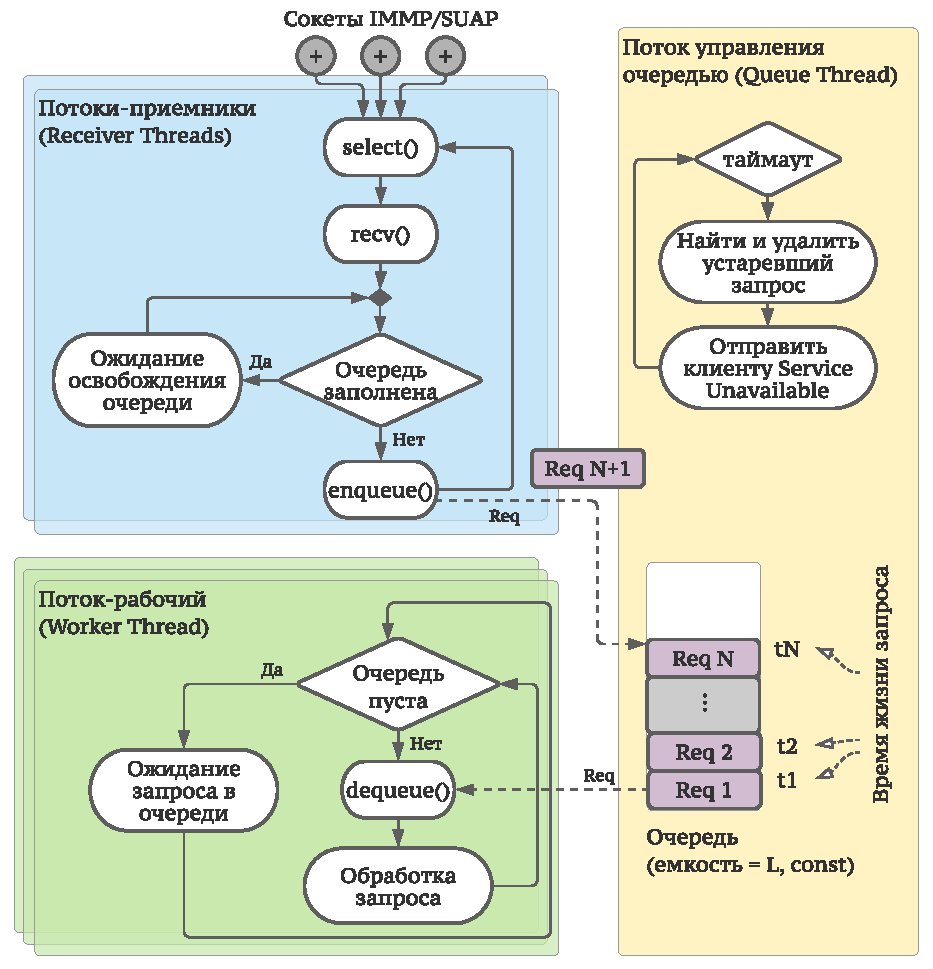
\includegraphics [width=0.75\textwidth] {chapter5/ch5_svrd_threads}
  }
  \caption{Архитектура супервизора SVRD}
  \label{fig:ch5_svrd_threads}
\end{figure}

Нагрузка на супервизор может быть достаточно высокой, особенно если в системе содержится несколько радиомодулей (и, соответственно, несколько модулей G2RD) и множество приложений. Для обеспечения масштабируемости SVR спроектирован многопоточным: все запросы, поступающие по IMMP или SUAP, поступают в очередь, откуда извлекаются и обрабатываются потоками-рабочими. Число потоков-рабочих можно настраивать. Взяв запрос, рабочий обрабатывает его синхронно. Если при этом требуется обратиться к другому модулю, он сам отправляет запрос этому модулю по IMMP и дожидается ответа. Из-за этой особенности реализации даже при небольшой загрузке целесообразно использовать несколько потоков-рабочих (по-умолчанию, в системе используется 9 рабочих). Упрощенная программная архитектура супервизора показана на рис.~\ref{fig:ch5_svrd_threads}.

Попав в очередь, запрос не ждет бесконечно долго, пока рабочий не освободится. Вместо этого в системе определено максимальное время ожидания обслуживания, по истечении которого запрос удаляется из очереди. Отслеживанием истечения времени ожидания занимается отдельный поток, управляющий очередью (см. рис.~\ref{fig:ch5_svrd_threads}). Очередь имеет фиксированную емкость.

Управление перегрузками в системе реализовано на стороне отправителя. Если очередь заполнена, поток-приемник ждет освобождения места без ограничения времени. Так как у всех запросов есть предельные времена ожидания, рано или поздно место в очереди освободится, поток-приемник не зависнет навсегда. Отправитель IMMP- или SUAP-запроса ждет ответа в течение ограниченного времени. Если ответа в течение этого времени не приходит, он сигнализирует о перегрузке системы. Таким образом, результат обработки, отправленный слишком поздно, будет просто проигнорирован.

Отметим, что особенность помещения запросов в очередь, когда поток-приемник ждет освобождения очереди, может быть оптимизирована в следующих версиях системы: желательно синхронизировать предельное время нахождения запроса на стороне приемника (и в очереди, и до этого, в ожидании освобождения очереди) с предельным временем ожидания ответа отправителем запроса. Это позволит быстрее снижать нагрузку при перегрузке, удаляя устаревшие запросы еще до их попадания в очередь. В качестве альтернативы, можно передавать отправителю ответ с кодом 411 (Not Ready) сразу при обнаружении заполненной очереди потоком-приемником.

Супервизор хранит конфигурацию других модулей, которые он передает в сообщении IMMP ACK при подключении к нему (см. рис.~\ref{fig:ch5_immp_session}). Если во время работы настройки модуля меняются, они хранятся в конфигурации времени исполнения и сбрасываются при перезапуске модуля. Для переноса параметра из конфигурации времени исполнения в хранимую конфигурацию на супервизоре нужно выполнить процедуру <<system.store-config>>, передав соответствующий CALL-запрос.


%%% --------------------------------------------
\subsection{RFID-адаптер G2RD}\label{sec:ch5_components_g2rd}
%%% --------------------------------------------

Модуль RFID-адаптера (G2RD) осуществляет взаимодействие с радиомодулем RFID. Он поддерживает два протокола: IMMP (в роли клиента) и ITOP (в роли сервера). Как и другие модули системы, после включения он подключается по IMMP к супервизору и получает от него стартовую конфигурацию, а в дальнейшем получает от супервизора запросы на получение или изменение параметров и вызов процедур. По протоколу ITOP к G2RD подключаются другие модули (TFPD, веб-интерфейс и прочие), которым нужно выполнить те или иные операции над метками.

\begin{figure}[ht]
  \centerfloat{
    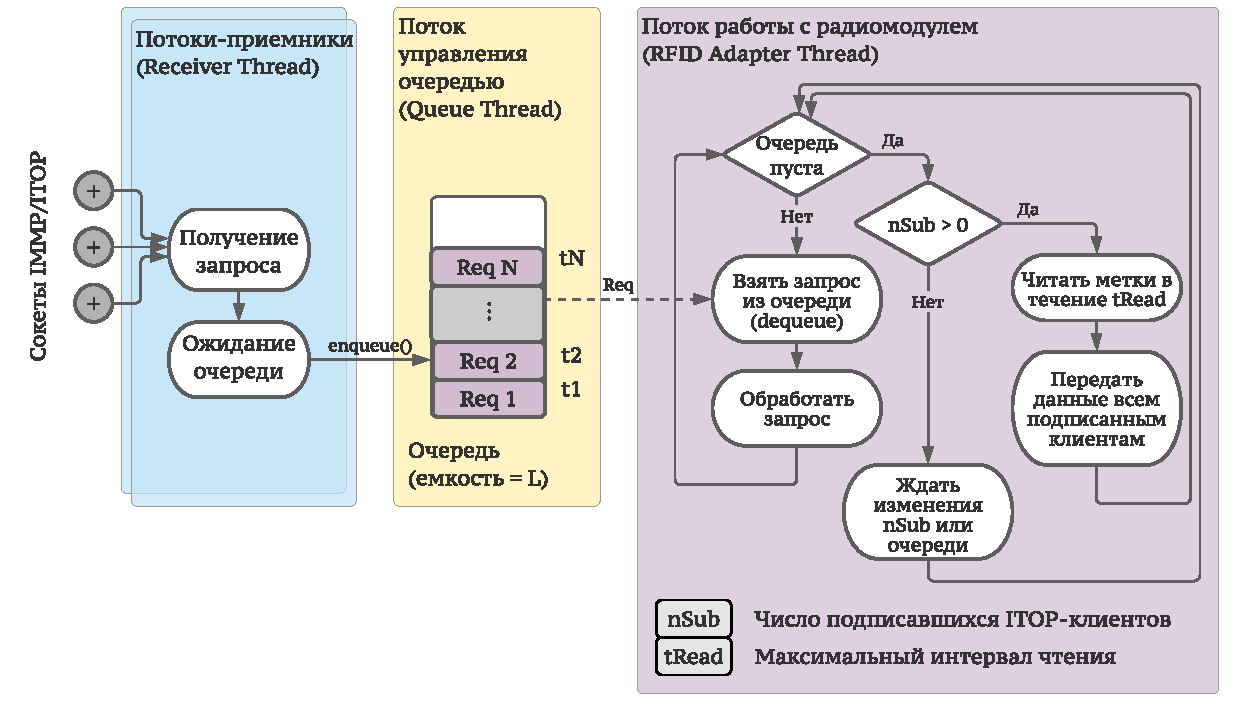
\includegraphics [width=1.0\textwidth] {chapter5/ch5_g2rd_threads}
  }
  \caption{Архитектура RFID-адаптера G2RD}
  \label{fig:ch5_g2rd_threads}
\end{figure}


Основная сложность в реализации G2RD заключается в том, что сам радиомодуль RFID может одновременно выполнять только одну операцию (читать или записать метку, получить или установить параметр). То есть радиомодуль является разделяемым ресурсом, доступ к которому должен быть синхронизирован. Если другой модуль подписался на поток меток, и радиомодуль будет постоянно занят чтением, то запросы на его настройку или запись меток не смогут быть выполнены до тех пор, пока подписка не будет остановлена, что не всегда возможно. Так как запросы к G2RD по IMMP приходят от потоков-рабочих супервайзера, которые работают синхронно, блокировка запросов в G2RD привела бы каскадно к повышению загрузки SVR "--- его потоки-рабочие были бы заблокированы до истечения предельного времени обработки запроса. Для того, чтобы избежать такой ситуации и дать возможность работать со считывателем одновременно различным модулям, потребовалось обеспечить приоритизацию операций.

На рис.~\ref{fig:ch5_g2rd_threads} показана архитектура RFID-адаптера. Потоки-приемники и поток управления очередью схожи с аналогичными потоками, используемыми в SVR (см. рис.~\ref{fig:ch5_svrd_threads}). Потоки-приемники получают, десериализуют и помещают в очередь запросы, пришедшие по протоколам IMMP и ITOP, а поток управления очередью отслеживает устаревшие запросы и удаляет их. Поток-рабочий, который обрабатывает запросы, в G2RD один, так как именно он обеспечивает взаимодействие с радиомодулем. Этот поток отслеживает число подписок, интервалы чтения, указанные запросах ITOP SUBSCRIBE, и ведет учет подписавшихся ITOP-сессий. Если в очереди есть хотя бы один запрос, поток-рабочий выполняет его. Если запросов нет, но есть активные подписки, поток-рабочий инициирует чтение в течение кванта времени. Этот квант выбирается максимальным среди всех квантов, указанных в запросах SUBSCRIBE, и не превосходит 500~мс. После окончания чтения, поток опять проверяет очередь запросов и продолжает чтение только в том случае, если очередь по-прежнему пуста. Таким образом исключается блокировка на непрерывном чтении, а обработка запросов приобретает более высокий приоритет. Если очередь пуста и подписок нет, поток спит до тех пор, пока не появятся запросы или подписки. В это время радиомодуль RFID неактивен и не расходует энергию.


%%% --------------------------------------------
\subsection{Приложение TFPD и клиент TFPC}\label{sec:ch5_components_tfpd_tfpc}
%%% --------------------------------------------

Модуль-приложение TFPD используется в качестве прокси-сервера между клиентами, подключающимися по протоколу TFP, и RFID-адаптером, с которым TFPD взаимодействует по протоколу ITOP (см. рис.~\ref{fig:ch5_tfp_session_2}). Приложение TFPD позволяет снять часть нагрузки с RFID-адаптера, так как при подключении нескольких клиентов оно будет поддерживать единственную сессию с RFID-адаптером и отправлять данные во все клиентские TFP-сессии. Как и другие модули системы, начальную конфигурацию TFPD получает от SVR сразу после включения и подключения к SVR по протоколу IMMP. Конфигурация TFPD включает, среди прочего, максимальное число одновременных клиентстких соединений.

В состав системы входит утилита TFPC, выполняющая функции клиента TFP. Она позволяет подключаться к TFPD и записывать полученные метки в базу или файл. Основное назначение TFPC "--- подключение к системе управления из внешней информационной системы и запись прочитанных меток в базу данных, однако она также может быть использована для кэширирования меток на считывателе. Такое решение использовалось, в частности, в ходе эксперимента в городе Казань, когда сеть периодически оказывалась перегружена данными с видеокамер, и соединение с центром обработки данных обрывалось.

Изначально TFPC, как и остальные модули системы, был реализован на языке C++. При подготовке к эксперименту в 2020 году была также выполнена его реализация на языке Python 3.



%%% --------------------------------------------
\subsection{Утилита UAX и интерфейсы управления}\label{sec:ch5_components_uax_and_cli}
%%% --------------------------------------------

В системе были реализованы два интерфейса управления: веб-интерфейс и интерфейс командной строки. Обоим интерфейсом нужно отрпавлять супервайзеру по протоколу SUAP запросы на получение или установку параметров модулей и запрашивать удаленное выполнение процедур, а также взаимодействовать с RFID-адаптером по протоколу ITOP. Обработка команд в любом из интерфейсов управления сводится к четырем шагам: проверке корректности аргументов команды, формированию и отправке запроса по SUAP или ITOP, ожиданию ответа от SVR или G2RD соответственно и выводу результата пользователю. Для унификации и упрощения разработки интерфейсов управления была реализована утилита UAX (User Agent Executor), которая в качестве аргумента получает строку с командой, обменивается данными с нужным модулем системы и выводит результат в поток стандартного вывода. Таким образом, любому интерфейсу достаточно сформировать строку с командой, запустить утилиту UAX в отдельном процессе и получить результат в его выводе, а по коду завершения определить успешность выполнения команды.

Команды UAX имеют вид  <<\textit{операция}:[\textit{модуль}.\textit{объект}|\textit{действие}] \textit{аргументы}>>, где <<\textit{операция}>> "--- одна из строк <<\textbf{get}>>, <<\textbf{set}>>, <<\textbf{call}>>, <<\textbf{rfid}>>, <<\textbf{login}>> или <<\textbf{logout}>>. Операции <<\textbf{get}>>, <<\textbf{set}>> и <<\textbf{call}>> должны включать адрес в виде названия модуля и имени объекта, например <<tfpd.conns-num>> (число подключений к TFPD) или <<g2rd.power-read>> (мощность, на которой радиомодуль читает метки). Операция <<\textbf{rfid}>> должна включать одно из доступных действий: <<\textbf{subscribe}>>, <<\textbf{readmem}>>, <<\textbf{writemem}>> или <<\textbf{writeepc}>>. Во всех командах после описания действия и адреса объекта нужно передать список аргументов в формате <<\textit{ключ}=\textit{значение}>>: в команде <<\textbf{login}>> нужно передать имя пользователя и пароль, а во всех остальных "--- как минимум ключ <<\textbf{skey}>>, который был получен с помощью команды <<\textbf{login}>>. Результаты выполнения команд выводятся в стандартный поток. Всем операциям кроме <<\textbf{rfid}>> соответствуют запросы SUAP (см. раздел~\ref{sec:ch5_suap}), а операции <<\textbf{rfid}>> "--- запросы ITOP (см. раздел~\ref{sec:ch5_itop}), соответствующие выбранному действию. Отметим, что команда <<\textbf{rfid}:\textbf{subscribe}>> позволяет читать метки только в течение ограниченного времени, от 200 до 1000 миллисекунд, за счет установки заголовка <<Continuous: false>> в сообщении ITOP SUBSCRIBE (см. рис.~\ref{fig:ch5_itop_session_2}).

В следующем примере администратор подключается к SVRD, получает ключ SKey и запрашивает число текущих подключений к TFPD, температуру радиомодуля и мощность считывателя. Затем он изменяет текущую мощность считывателя и сохраняет новое значение, чтобы оно использовалось после перезагрузки. После этого пользователь завершает сессию.

\begin{lstlisting}[language=Bash]
$ uax "login: username=admin password=qwerty"
42
# Получить число активных подключений к TFPD:
$ uax "get:tfpd.conns-num skey=42"
tfpd.conns-num: 1
# Получить температуру радиомодуля:
$ uax "get:g2rd.temperature skey=42"
g2rd.temperature: 27
# Получить текущую мощность радиомодуля (100*дБм):
$ uax "get:g2rd.power-read skey=42"
g2rd.power-read: 2900  # 29 дБм
# Установить значение мощности чтения радиомодуля:
$ uax "set:g2rd.power-read skey=42 value=3150"
$ uax "get:g2rd.power-read skey=42"
g2rd.power-read: 3150  # 31.5 дБм
# Сохранить новое значение мощности радиомодуля
$ uax "call:system.store-config skey=42 plist=g2rd.power-read"
# Выйти из системы (сделать невалидным ключ):
$ uax "logout: skey=42"
\end{lstlisting}



%%%%%%%%%%%%%%%%%%%%%%%%%%%%%%%%%%%%%%%%%%%%%%%%%%%%%%%%%%%%%%%%%%%%%%%%%%%%%%%%
\section{Реализация RFID-считывателей и системы управления}\label{sec:ch5_implementation}
%%%%%%%%%%%%%%%%%%%%%%%%%%%%%%%%%%%%%%%%%%%%%%%%%%%%%%%%%%%%%%%%%%%%%%%%%%%%%%%%

%%% --------------------------------------------
\subsection{Аппаратная реализация считывателей}\label{sec:ch5_implementation_hardware}
%%% --------------------------------------------
Экспериментальные RFID-считыватели были выпущены во всепогодном исполнении с питанием через Ethernet (PoE). К каждому считывателю можно подключить до четырех антенн.

\begin{figure}[ht]
  \centerfloat{
    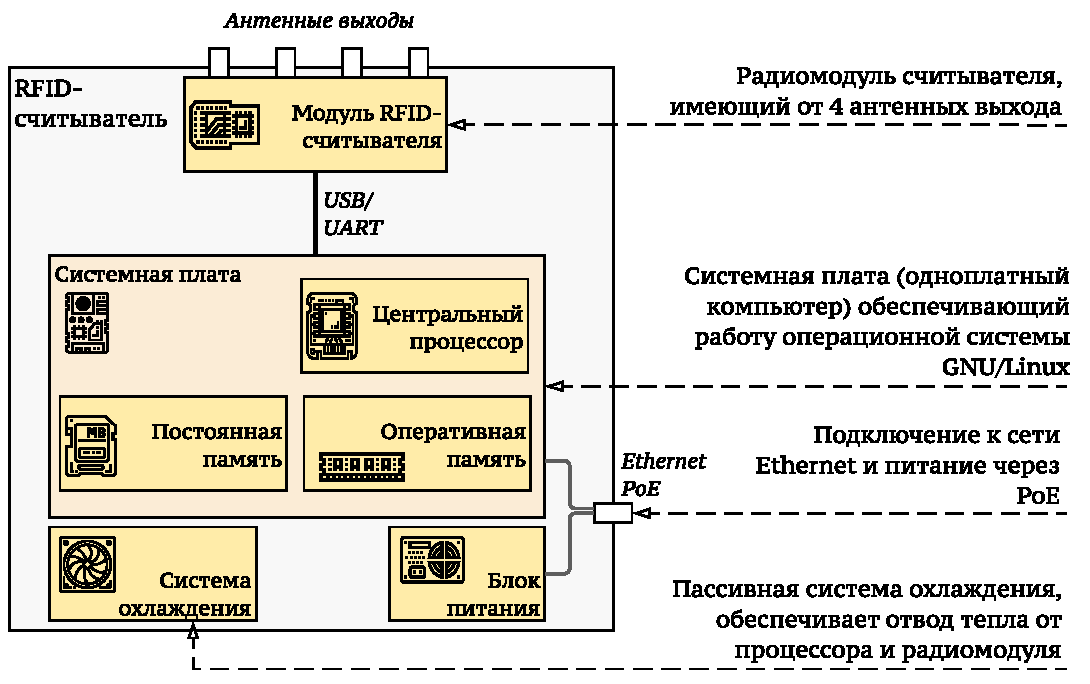
\includegraphics [width=0.85\textwidth] {chapter5/ch5_reader_hardware}
  }
  \caption{Аппаратная структура RFID-считывателя}
  \label{fig:ch5_reader_hardware}
\end{figure}

Аппаратная структура считывателя показана на рис.~\ref{fig:ch5_reader_hardware}. Считыватель состоит из одноплатного компьютера, радиомодуля RFID и модуля питания. Из-за всепогодного исполнения использовалось пассивное охлаждение, тепло от радиомодуля и процессора отводилось через радиатор на металлический корпус. Одноплатный компьютер построен на четырехядерном процессоре Exynos4412 Prime 1,7~ГГц ARM Cortex-A9, имеет 2~ГБ оперативной памяти LP-DDR2, интерфейс FastEthernet 100~Мб/с и сменную карту постоянной памяти на 8~ГБ. Питание осуществлялось через интерфейс Ethernet. Раидомодуль RFID имеет четыре антенных порта, он подключается к управляющему компьютеру через интерфейс USB. Модуль обеспечивает выходную мощность до 31,5~дБм.



%%% --------------------------------------------
\subsection{Особенности программной реализации}\label{sec:ch5_implementation_software}
%%% --------------------------------------------
Все описанные ранее в разделах \ref{sec:ch5_protocols} и \ref{sec:ch5_components} программные модули и протоколы,  кроме веб-интерфейса и части RFID-адаптера, взаимодействующей со считывателем, были реализованы на языке C++. Часть RFID-адаптера, работающая непосредственно с радиомодулем считывателя, была реализована на C. Для реализации web-интерфейса использовался фреймворк Flask на языке Python 3.

Все компоненты системы работают под управлением операционной системы Arch Linux. Для взаимодействия с сервисами оперционной системы (например, настройки сетевого адаптера, журнала syslog или перезагрузки) были написаны скрипты на языках Bash и Python, которые вызываются SVR при обращении к соответствующим процедурам или свойствам. Например, для получения текущего IP-адреса считывателя нужно отправить запрос IMMP GET <<system.network-address>> на SVR. Получив его, поток-рабочий в SVR выполнит в отдельном процессе скрипт, который просмотрит текущие сетевые интерфейсы и вернет IP-адрес, связанный с интерфейсом Ethernet. Для установки статического IP-адреса нужно передать команду IMMP CALL <<system.network-setup-static>> с параметрами <<address>>, <<netmask>> и <<gateway>>, получив которую SVR выполнит другой скрипт, настраивающий IP-адрес, маску и шлюз. За счет такого подхода систему достаточно просто адаптировать под разные дистрибутивы Linux, в которых могут использоваться различные версии системных служб. Так, система была успешна портирована на Ubuntu и Armbian.

Выделим несколько особенностей, общих для всех модулей кроме веб-интерфейса, реализованного на Python. Во-первых, в реализациях очередей, клиентов и серверов практически не используется динамическая память (функции \texttt{malloc}/\texttt{free}, операторы \texttt{new}/\texttt{delete}, функции \texttt{make\_shared<T>()} и пр.). Вместо этого под каждое сообщение или очередь заранее статически выделяется область памяти, заведомо превышающая предельно допустимый размер хранимого объекта. Этот подход позволяет не только повысить производительность за счёт отсутствия работы с выделением и освобождением памяти, но и существенно повысить надёжность за счёт снижения вероятности появления ошибок утечки памяти или обращений к ранее освобождённой памяти.

Во-вторых, большинство модулей, включающих серверы каких-либо протоколов (IMMP, ITOP и пр.), имеют в своем составе очереди, с помощью которых обработка запросов от различных клиентов мультиплексируется и может осуществляться даже одним потоком. Опрос сокетов также производится с мультиплексированием с помощью функции \texttt{pselect}.

В-третьих, все модули реализованы в виде многопоточных приложений с использованием библиотеки pthreads (POSIX Threads).

При разработке модуля G2RD требовалось использовать программный интерфейс радиомодуля, написанный на языке C. Для того, чтобы иметь возможность быстрой замены модулей, была разработана промежуточная библиотека (также на языке C), реализующая основные функции: чтение метки в течение заданного интервала, запись значения EPCID на метку, запись значения в заданный банк памяти, получение и запись значений параметров радиомодуля. Эту библиотеку несложно адаптировать к новым радиомодулям, при наличии соответствующей спецификации протокола взаимодействия или API.




%%%%%%%%%%%%%%%%%%%%%%%%%%%%%%%%%%%%%%%%%%%%%%%%%%%%%%%%%%%%%%%%%%%%%%%%%%%%%%%%
\section{Экспериментальные испытания}\label{sec:ch5_experiments}
%%%%%%%%%%%%%%%%%%%%%%%%%%%%%%%%%%%%%%%%%%%%%%%%%%%%%%%%%%%%%%%%%%%%%%%%%%%%%%%%

В общей сложности было проведено три экспериментальных испытания разработанной системы радиочастотной идентификации автомобилей. Первое масштабное испытание системы состоялось в 2014--2015 годах, когда в городе Казань более 700 автобусов были оснащены метками, на улицах установлены считыватели и в течение нескольких зимних месяцев производилась регистрация проездов. Следующий эксперимент состоялся весной 2020 года на полигоне в Казани, в нем проверялась успешность идентификации автомобилей, едущих со скоростями до 170 км/ч, совершающими обгон и прочие маневры. Наконец, третий эксперимент начался летом 2021 года на платном участке центральной кольцевой автодороги вокруг Москвы (ЦКАД), в нем метками были оснащены 9 автомобилей аварийных комиссаров. Цель последнего эксперимента "--- проверить применимость UHF RFID в системе бесконтактной оплаты проезда по платной дороге. На момент написания диссертации этот эксперимент еще не завершен.


%%% --------------------------------------------
\subsection{Испытания в Казани в 2014 году}\label{sec:ch5_experiments_kazan2014}
%%% --------------------------------------------

В конце осени 2014 года был запущен большой эксперимент в городе Казань (республика Татарстан). В ходе эксперимента номерами с радиометками были оснащены 740 автобусов и были оборудованы четыре точки радиочастотной идентификации. Оборудование для двух из них было разработано коллективом при активном участии автора (проектирование архитектуры системы управления и протоколов; разработка программного обеспечения системы управления; установка, настройка программ в ЦОДе и настройка считывателей; анализ полученных результатов и расчёт вероятности идентификации).

\begin{figure}[ht]
  \centerfloat{
    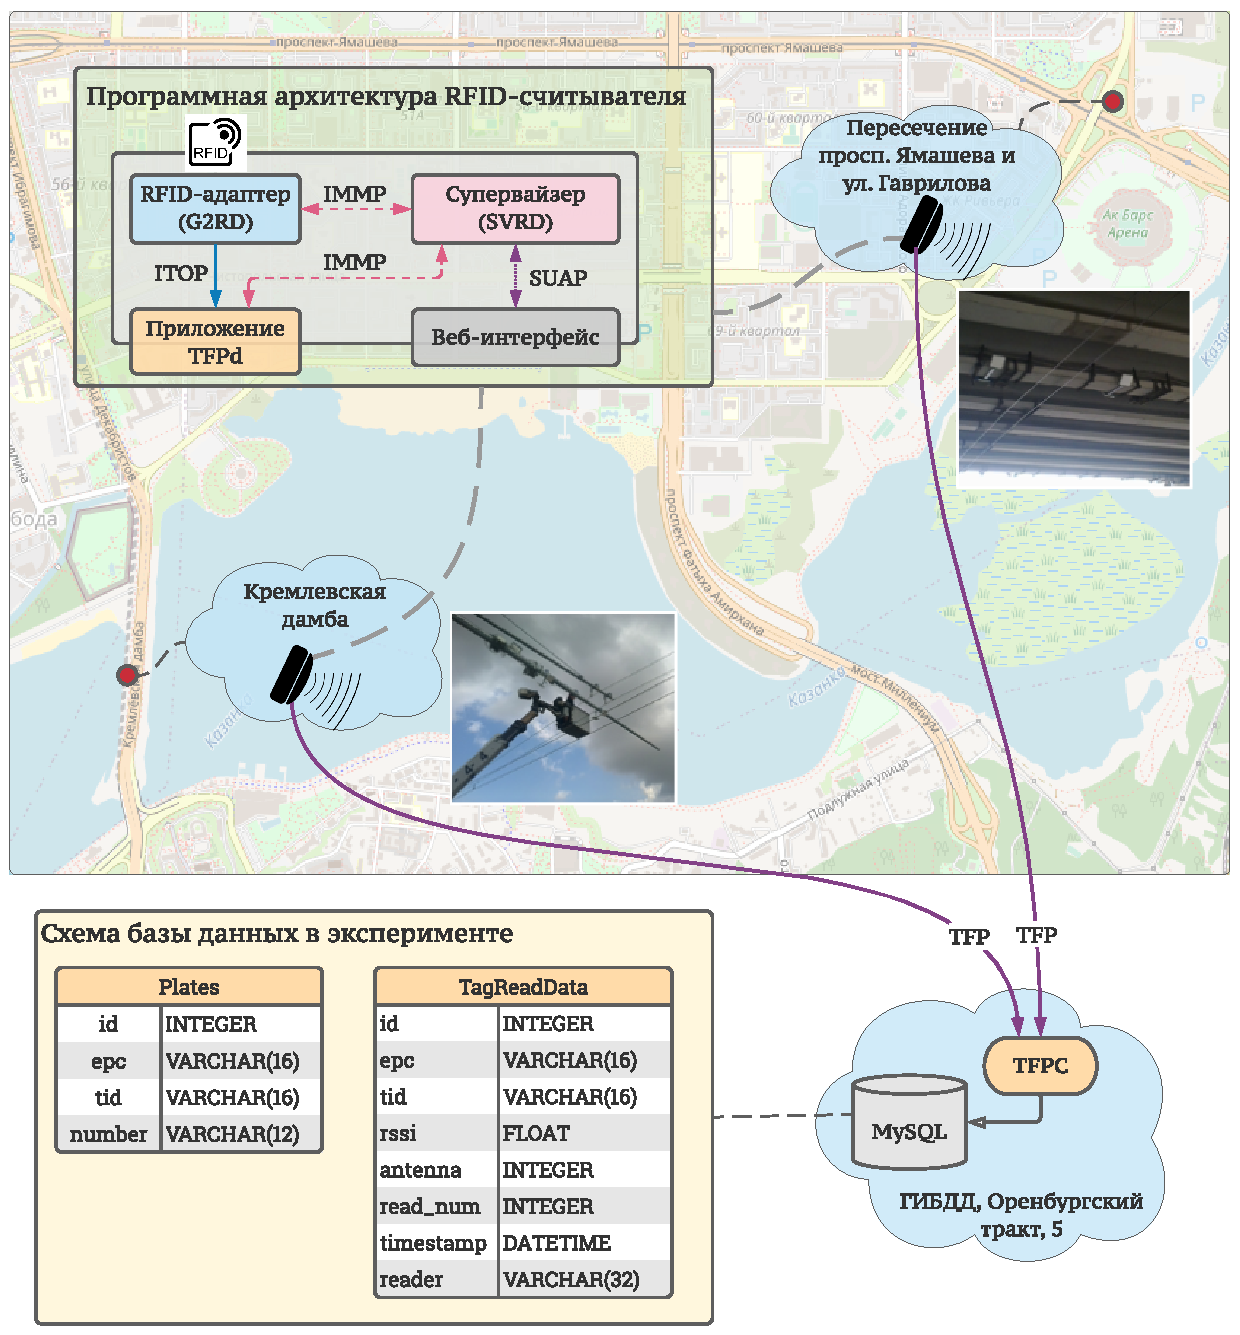
\includegraphics [width=0.95\textwidth] {chapter5/ch5_kazan2014_schema}
  }
  \caption{Схема размещения считывателей и программных компонентов распределенной системы в Казани в 2014 году}
  \label{fig:ch5_kazan2014_schema}
\end{figure}

Каждый считыватель оснащался четырьмя антеннами, по две антенны на каждую из полос. Одна антенна в каждой паре была направлена на чтение передних номеров, вторая "--- задних. Угол наклона антенн был приблизительно равен 45\textdegree. Считыватели размещались на тех же опорах, на которых были установлены камеры видеофиксации: на Кремлевской дамбе на штанге над дорогой, на высоте 5,8~м, а на пересечении ул. Гаврилова и просп. Ямашева "--- под сводом путепровода, немного ниже.

Номера с метками для этого эксперимента были разработаны немецкой компанией Tonnjes Group и выпущены российской фирмой ООО <<Знак>>. Чипы меток были производства компании NXP. На метках были записаны уникальные значения EPCID, а для повышения достоверности использовалась идентификация и по EPCID, и по TID. Номера TID на метках имели калсс E0~\cite{StdGen2}, то есть первые 8 бит содержали шестнадцатиричное значение E0, следующие 8 бит "--- код производителя, а последние 48 бит "--- уникальный номер метки.

Схема размещения считывателей и программных компонентов показана на рис.~\ref{fig:ch5_kazan2014_schema}. На считывателях были установлены супервайзеры (SVR), приложения TFPD, RFID-адаптеры и веб-серверы. Сервер был размещен в центре обработки данных (ЦОД) ГИБДД города Казань, подключение к считывателям происходило посредством протокола TFP.  На сервере в ЦОД был установлен клиент TFPC и база данных MySQL, в которую записывались прочитанные метки. Позднее на считыватели пришлось добавить модули TFPC для кэширования "--- из-за перегрузок в сети (она использовалась для передачи видеотрафика от камер) TFP-соединения часто разрывались и данные терялись. Для каждой метки в базу данных записывались время, идентификатор считывателя, значения EPC и TID, уровень сигнала от метки, число прочтений, номер антенны. Также в отдельной таблице хранились соответствия значений TID и номерных знаков, поэтому была возможность выгрузки информации о времени проезда автобусов напрямую из базы данных. Схема базы данных приведена на рис.~\ref{fig:ch5_kazan2014_schema}.

Эксперимент длился до начала 2015 года, в течение поздней осени и зимы. Задачей эксперимента было практически обосновать применимость технологии радиочастотной идентификации для регистрации проездов автомобилей на нормальных скоростях в условиях городского потока при плохих погодных условиях.

\begin{table}[!t]
	\renewcommand{\arraystretch}{1.3}
	\caption{Параметры RFID-считывателей в Казани в 2014 году.}
	\label{table:ch5_kazan_rfid_settings}
	\centering
	\begin{tabular}{|l|l|}
		\hline
		Параметр                                   & Значение   \\\hline
		Интервал Tari                              & 12,5~мкс   \\
		Показатель числа слотов (Q)                & 2          \\
		Число символов на бит (M)                  & 4          \\
		Использовать расширенную преамбулу (TRext) & 0 (нет)    \\
		Длина EPCID                                & любая      \\
		Длина TID                                  & 64 бита    \\
		Сессия                                     & S0         \\
		Флаг опроса меток                          & Всегда A   \\
    Выходная мощность радиомодуля              & 31,5~дБм   \\
    Усиление антенн                            & 8~дБ       \\
    Общие потери в кабелях и разъемах          & 2,6~дБ     \\\hline
	\end{tabular}
\end{table}

Параметры настройки радиомодулей RFID-считывателей приведены в табл.~\ref{table:ch5_kazan_rfid_settings}. Отметим две особенности. Во-первых, у меток всегда читались ровно 64 бита (4 машинных слова) банка TID, а длина значения EPCID не ограничивалась. Во-вторых, опрос всегда проводился по флагу A. Как показали более поздние исследования, результаты которых были приведены в главе 3, это не всегда оптимальная стратегия, и можно немного улучшить идентификацию, если периодически инвертировать флаг. В то же время, считыватели периодически переключали антенны, поэтому сброс питания так или иначе производился. Настройки параметров Q, Tari и M оказались достаточно удачными, что позднее было показано и теоретически (см. главу 2).

Для оценки вероятности идентификации на протяжении нескольких дней силами ГИБДД Казани были собраны данные о проездах автобусов, с помощью визуального наблюдения. Эти данные обрабатывались и сравнивались с информацией, полученной от считывателей, с поправкой на погрешности (например, время могло немного отличаться). Результаты несколько различались между точками и составили от 92~\% идентифицированных транспортных средств на Кремлевской дамбе до 96~\% на пересечении ул. Гаврилова и просп. Ямашева. Еще одно наблюдение из эксперимента "--- в 2014 году практически все считанные метки были метками в номерах, то есть прочтения <<случайных>> меток были очень редкими и при выборе параметра Q можно было руководствоваться тем, что коллизии практически не происходят даже при малом числе слотов. Как показали более поздние эксперименты, которые будут описаны далее, к 2021 году это предположение перестало быть верным.

Следует отметить, что одной из основных проблем при проведении эксперимента оказалась высокая перегруженность оптических каналов связи между считывателями и центром обработки данных, которые также использовались для передачи уличного видеонаблюдения. Перегрузки приводили к тому, что значительную часть времени соединений между считывателями и сервером не было, но за счет использования кэширования удалось избежать потери данных о проездах. В то же время, для реального использования системы радиочастотной идентификации и обеспечения оперативного воздействия при обнаружении нарушений правил дорожного движения или, например, выявления похищенных автомобилей может требоваться либо предоставление гарантированной пропускной способности в существующих проводных каналах, либо построение беспроводных многошаговых сетей.


%%% --------------------------------------------
\subsection{Испытания в Казани в 2020 году}\label{sec:ch5_experiments_kazan2020}
%%% --------------------------------------------

Следующие испытания состоялись в Казани в 2020 году на полигоне ИТС ООО <<Казань-Телематика>> в рамках НИР по применению RFID для идентификации транспорта. Эти испытания длились несколько дней, их целью было проверить работоспособность системы при проезде автомобилей на высоких скоростях и при совершении маневров. Метки для этого эксперимента были произведены АО <<Микрон>>.


\begin{figure}[ht]
  \centerfloat{
    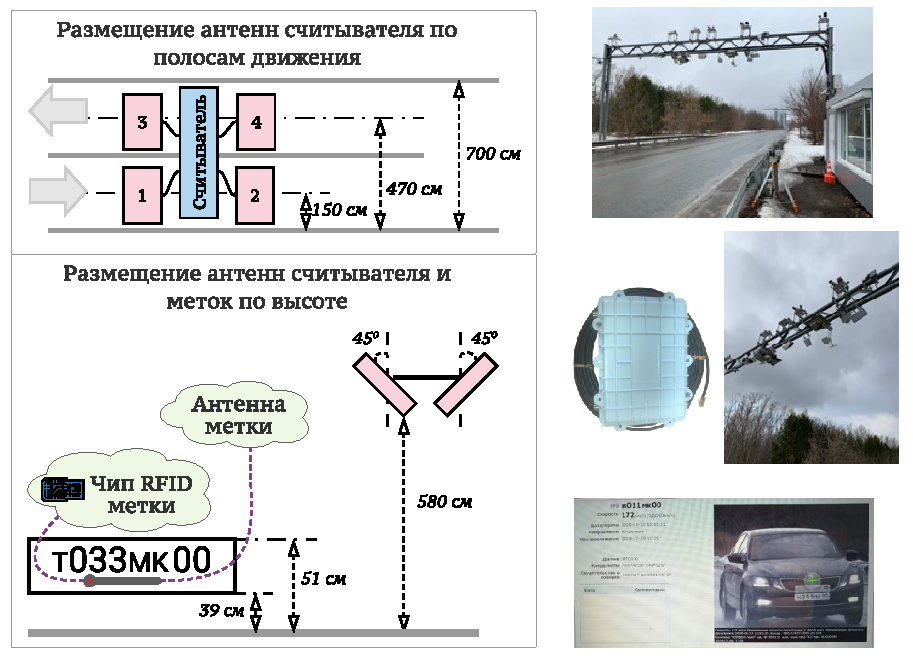
\includegraphics [width=0.8\textwidth] {chapter5/ch5_kazan2020_schema}
  }
  \caption{Схема размещения RFID-оборудования в Казани в 2020 году}
  \label{fig:ch5_kazan2020_schema}
\end{figure}

Считыватель размещался на той же опорной конструкции, на которой размещены системы видеофиксации нарушений. Схема расположения антенн считывателя, а также размещение метки на номерном знаке и фотографии с полигона приведены на рис.~\ref{fig:ch5_kazan2020_schema}. Настройки считывателя были теми же, что и в эксперименте 2014 года (см. табл.~\ref{table:ch5_kazan_rfid_settings}).

Во время эксперимента проверялась успешность идентификации метки при проезде с заданной скоростью от 40~км/ч до 170~км/ч (самый быстрый проезд был на скорости 172~км/ч), при обгоне одним автомобилем другого и при следовании автомобилей друг за другом в потоке. Во всех случаях метки были успешно идентифицированы. Для точного измерения скорости движения использовался комплекс <<Кордон-М>> фирмы ООО <<Симикон>>.

В отличие от предыдущего эксперимента 2014 года, метки АО <<Микрон>> в этом эксперименте имели класс E2~\cite{StdGen2}, то есть первый байт содержал шестнадцатиричное значение E2, следюущие три бита "--- служебные флаги, потом 9-битный идентификатор производителя MDID (Mask Designer Identifier), 12-битный номер модели и уже после него уникальный номер метки. Общая длина идентификатора, таким образом, составляла 96 бит (6 машинных слов). К сожалению, эта особенность стала известна уже во время эксперимента, поэтому различить метки по TID не удалось "--- первые 64 бита у всех меток совпадали. В дальнейшем эта проблема была исправлена и уже в следующем эксперименте считыватели были настроены на 96-битные TID.

\begin{figure}[ht]
  \centerfloat{
    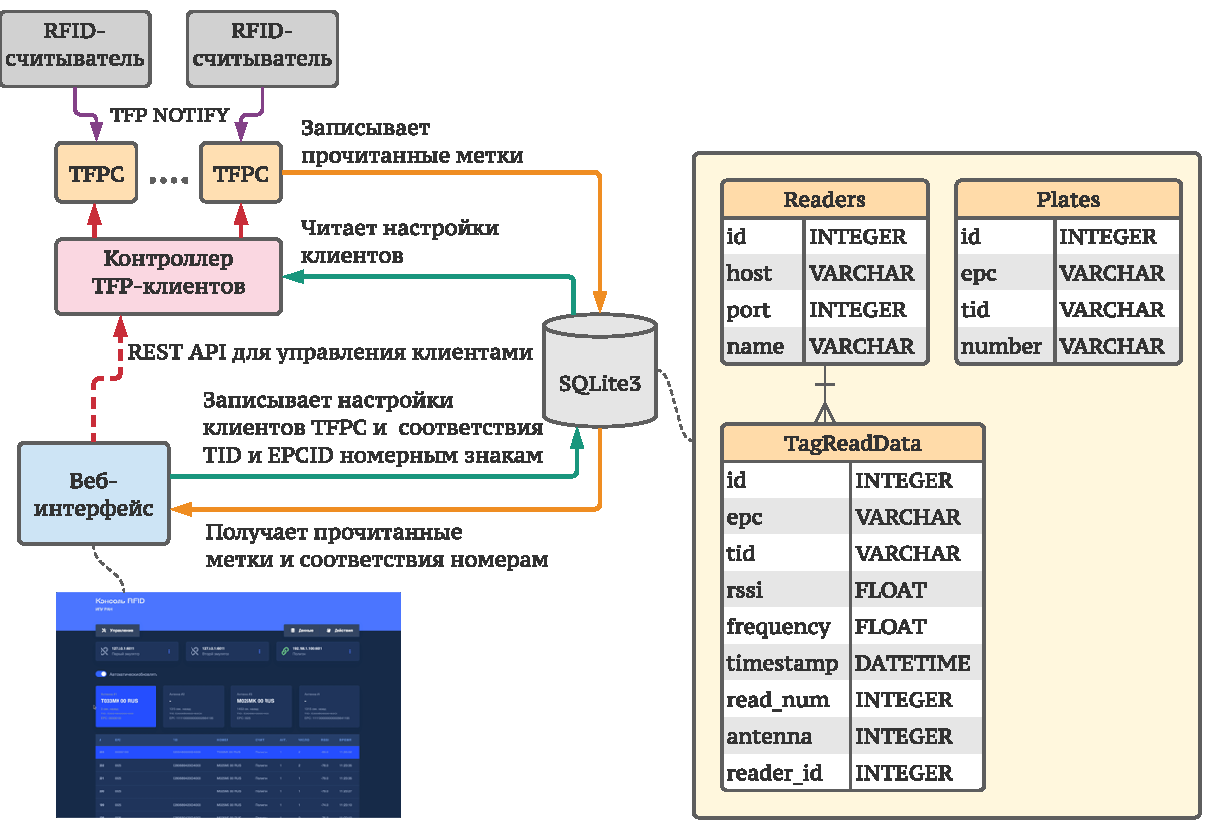
\includegraphics [width=0.95\textwidth] {chapter5/ch5_kazan2020_client}
  }
  \caption{Схема клиентского программного обеспечения для испытаний}
  \label{fig:ch5_kazan2020_client}
\end{figure}

Также для эксперимента потребовалось реализовать более функциональную клиентскую часть, позволяющую настраивать клиентов TFPC и получать статистику проездов через веб-интерфейс. Схема программного обеспечения и упрощенная модель данных показаны на рис.~\ref{fig:ch5_kazan2020_client}. Вся клиентская часть была построена на языке Python 3. Она включала клиентов TFPC, которые создавались динамически контроллером TFP-клиентов. Для взаимодействия между TFP-клиентами и контроллером использовался простой бинарный протокол. Параметры подключения контроллер получал из базы данных SQLite, в которую же записывали данные TFP-клиенты. Настройка считывателей и получение статистики проездов производилась через веб-интерфейс, реализованный на Flask. Для управления началом и остановкой чтения контроллер предоставлял программный интерфейс REST API, к которому подключался тот же веб-интерфейс.


%%% --------------------------------------------
\subsection{Испытания на платном участке ЦКАД в 2021 году}\label{sec:ch5_experiments_ckad2021}
%%% --------------------------------------------

Последние испытания начались в 2021 году на платном участке центральной кольцевой автодороги (ЦКАД) и проводились, как и в 2020 году, совместно с АО <<Микрон>>. Целью эксперимента являлась проверка возможности использования UHF RFID для оплаты проезда по платной дороге и проверка точности позиционирования идентифицируемых автомобилей. В рамках эксперимента оборудована одна точка идентификации считывателем с четырьмя антеннами над двумя полосами одного направления. Метки производства АО <<Микрон>> были установлены на 9 автомобилей службы аварийных комиссаров, периодически проезжающих по этому участку ЦКАД. В отличие от предыдущих экспериментов антенны считывателя были установлены на большей высоте.

В эксперименте использовалось то же оборудование и программное обеспечение на считывателе, что и в эксперименте в Казани 2020 года. С учетом особенностей меток, считыватель был настроен на чтение 96 бит TID. Изменения коснулись только клиентской части "--- вместо реализации TFPC на Python 3 была использована более эффективная и надежная реализация на C++, модель данных была расширена для учета связей антенн с полосами и направлениями движения, и вместо СУБД SQLite использовалась более производительная и надежная PostgreSQL.

Стоит отметить, что если в 2014 году сторонние, не участвующие в эксперименте, метки составляли не более 10~\% от всех прочитанных меток, то в 2021 году таких меток стало на несколько порядков больше. Так, за 26 дней эксперимента было прочитано более 63000 меток, и лишь 115 прочтений относились к меткам в номерах машин, используемых в эксперименте. Вероятно, остальные метки размещаются на упаковках товаров в кузовах фур, корпусах автомобилей или под лобовыми стекалми (например, для бесконтактного проезда на парковку или в дачные поселки).



%%%%%%%%%%%%%%%%%%%%%%%%%%%%%%%%%%%%%%%%%%%%%%%%%%%%%%%%%%%%%%%%%%%%%%%%%%%%%%%%
\section{Заключение}\label{sec:ch5_conclusion}
%%%%%%%%%%%%%%%%%%%%%%%%%%%%%%%%%%%%%%%%%%%%%%%%%%%%%%%%%%%%%%%%%%%%%%%%%%%%%%%%

В главе были представлены следующие результаты.

\begin{enumerate}
  \item Разработана распределенная система управления RFID-считывателями. Для управления и передачи данных в системе используются различные протоколы, позволяющие избежать перегрузки системы при увеличении числа RFID-считывателей. Система управления обладает высокой гибкостью, позволяет реализовывать на ее основе считыватели различной конфигурации.
  \item Проведены три экспериментальных испытания системы: в 2014 и в 2020 годах в Казани, и в 2021 году в Московской области на ЦКАД. Успешные результаты испытаний показывают, что разработанную систему радиочастотной идентификации можно использовать для регистрации автомобилей, движущихся с большими скоростями и совершающих различные маневры на дороге.
  \item Полученные результаты экспериментов согласуются с теоретическими результатами, представленными в диссертационной работе. Отмечено, что для эффективного использования системы желательно иметь выделенные каналы связи, для построения которых можно использовать многошаговые беспроводные сети.
\end{enumerate}


\clearpage
